%==============================================================================
%  Cross-Modal Attention Acts as a Frequency Filter
%  Why Verbose Prompts Improve Robustness in Vision-Language Models
%  Presentation deck — generated to match current paper state (2026-05-26)
%  All numbers verified against run JSONs; figures from paper/figures/.
%==============================================================================
\documentclass[aspectratio=169,11pt]{beamer}

\usetheme{metropolis}
\usepackage{amsmath,amssymb,amsthm}
\usepackage{graphicx}
\usepackage{booktabs}
\usepackage{array}
\usepackage{xcolor}
\usepackage{pifont}
\usepackage{tikz}
\usetikzlibrary{arrows.meta,positioning,calc,shapes.geometric,fit,backgrounds,decorations.pathreplacing}

\graphicspath{{figures/}}

% -------------------- Colour palette --------------------
\definecolor{pnavy}{HTML}{1F3A68}
\definecolor{paccent}{HTML}{D7552B}     % destabilising / Csem (complexity)
\definecolor{pgreen}{HTML}{2E7D55}      % stabilising / Cprompt (verbosity)
\definecolor{psoft}{HTML}{E8EEF4}
\definecolor{pgray}{HTML}{6B7280}
\definecolor{pgold}{HTML}{B08900}

\setbeamercolor{frametitle}{bg=pnavy, fg=white}
\setbeamercolor{progress bar}{fg=paccent}
\setbeamercolor{alerted text}{fg=paccent}
\setbeamercolor{title separator}{fg=paccent}
\metroset{sectionpage=progressbar, block=fill, numbering=fraction}

% -------------------- Math macros (match paper) --------------------
\newcommand{\Csem}{C_{\mathrm{sem}}}
\newcommand{\Cprompt}{C_{\mathrm{prompt}}}
\newcommand{\Cres}{C_{\mathrm{res}}}
\newcommand{\Hopt}{H_{\mathrm{opt}}}
\newcommand{\Wt}{W_t(\omega)}
\newcommand{\DF}{\Delta F(\omega)}
\newcommand{\Spred}{S_{\mathrm{pred}}}
\newcommand{\Gt}{G(t)}

% -------------------- Helper boxes --------------------
\newcommand{\keybox}[1]{%
  \begin{center}
  \begin{tikzpicture}
    \node[draw=paccent, line width=0.9pt, fill=paccent!6, rounded corners=4pt,
          inner sep=8pt, text width=0.92\linewidth] {#1};
  \end{tikzpicture}
  \end{center}}

\newcommand{\up}{\textcolor{paccent}{$\uparrow$}}
\newcommand{\down}{\textcolor{pgreen}{$\downarrow$}}
\newcommand{\cmark}{\textcolor{pgreen}{\ding{51}}}

% -------------------- Title --------------------
\title{\textbf{Cross-Modal Attention Acts as a Frequency Filter}}
\subtitle{Why Verbose Prompts Improve Robustness in Vision--Language Models}
\author{Anonymous ARR Submission}
\institute{}
\date{\small\textcolor{pgray}{Qwen3-VL \{2B, 8B\} \,\&\, LLaVA-OneVision \,$\cdot$\, GQA \& CLEVR \,$\cdot$\, 312k measurements/run}}

\begin{document}

%==============================================================================
\begin{frame}[plain]
  \titlepage
\end{frame}

%==============================================================================
\begin{frame}{One-sentence summary}
  \vfill
  \keybox{\large
    Cross-modal attention in a VLM forms a \textbf{task-conditioned frequency filter};
    its overlap with a corruption's spectrum \textbf{predicts drift}, and
    \textcolor{pgreen}{\textbf{verbose prompts broaden the filter to improve robustness}}.}
  \vfill
  \begin{center}
    \large\textcolor{paccent}{\textbf{Practical recipe: pad the prompt.}}
  \end{center}
  \vfill
\end{frame}

%==============================================================================
\section{Motivation}

\begin{frame}{Vision--language models are fragile under image corruption}
  \begin{columns}[T]
    \begin{column}{0.5\textwidth}
      A small image perturbation --- blur, JPEG, a few-pixel shift ---
      can flip a VLM's answer, even when a human sees no difference.

      \medskip
      \textbf{The puzzle:} the \emph{same image} and a \emph{semantically identical}
      question can be more or less robust depending only on \alert{how the
      question is worded}.

      \medskip
      We ask: \emph{what property of the prompt controls robustness,
      and why?}
    \end{column}
    \begin{column}{0.5\textwidth}
      \centering
      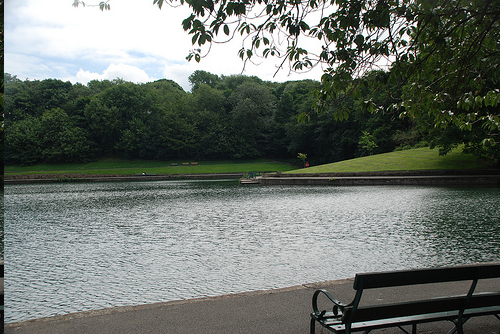
\includegraphics[width=\linewidth]{example_gqa_pert.png}\\
      \scriptsize\textcolor{pgray}{A GQA image under \texttt{Translation(+4)} --- our smallest geometric perturbation.}
    \end{column}
  \end{columns}
\end{frame}

\begin{frame}{Two opposite effects of question wording}
  \begin{columns}[T]
    \begin{column}{0.5\textwidth}
      \begin{block}{\textcolor{pgreen}{Verbosity $\Rightarrow$ more robust}}
        \emph{``Is there a cat?''}\\
        $\rightarrow$ \emph{``Please look carefully and answer: is there a cat?''}
        \medskip

        Same answer, \textbf{much smaller drift}.
      \end{block}
    \end{column}
    \begin{column}{0.5\textwidth}
      \begin{block}{\textcolor{paccent}{Complexity $\Rightarrow$ more fragile}}
        \emph{``Is there a cup?''}\\
        $\rightarrow$ \emph{``What colour is the cup left of the chair?''}
        \medskip

        Finer-grained reasoning, \textbf{larger drift}.
      \end{block}
    \end{column}
  \end{columns}
  \vfill
  \keybox{Both effects come from \textbf{one mechanism} --- a frequency filter induced by the prompt.}
\end{frame}

%==============================================================================
\section{The core idea}

\begin{frame}{Cross-modal attention as a frequency filter}
  \begin{columns}[T]
    \begin{column}{0.55\textwidth}
      The question's attention over image patches, projected into the 2D Fourier
      domain and radially binned, is a \textbf{distribution over spatial
      frequencies} --- the filter $\Wt$.

      \medskip
      \begin{itemize}
        \item Low bands $=$ coarse layout / shape
        \item High bands $=$ fine detail / texture
        \item \textcolor{pgreen}{Verbose prompts \textbf{widen}} $\Wt$
        \item \textcolor{paccent}{Fine reasoning \textbf{narrows}} $\Wt$
      \end{itemize}

      \medskip
      The answer \alert{drifts most} when the filter $\Wt$ and the corruption's
      spectrum $\DF$ sit on the \textbf{same frequencies}.
    \end{column}
    \begin{column}{0.45\textwidth}
      \centering
      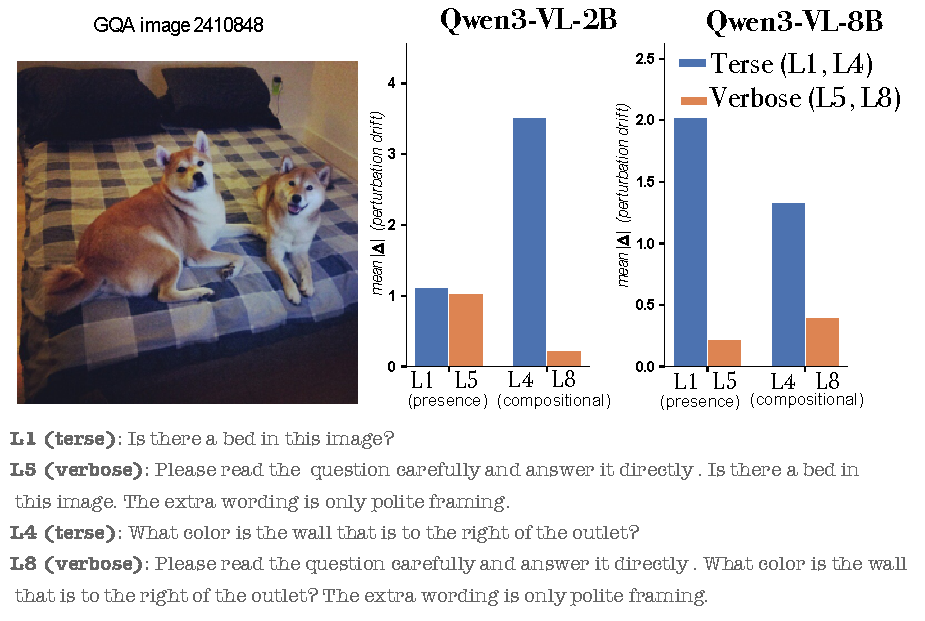
\includegraphics[width=\linewidth]{teaser_fig1_v2.pdf}\\
      \scriptsize\textcolor{pgray}{Verbose paraphrases cut drift variance across corruptions.}
    \end{column}
  \end{columns}
\end{frame}

\begin{frame}{The mechanism in one picture}
  \keybox{\centering
    \textbf{prompt} $\;\longrightarrow\;$ \textcolor{pnavy}{cross-modal attention}
    $\;\longrightarrow\;$ \textcolor{pnavy}{filter $\Wt$ over visual frequencies}\\[4pt]
    \textbf{corruption} $\;\longrightarrow\;$ \textcolor{pnavy}{spectral signature $\DF$}\\[6pt]
    \large\textbf{drift} $\;\propto\; \langle \Wt,\ \DF\rangle$ \quad
    \textcolor{pgray}{(spectral overlap)}}
  \vfill
  \begin{itemize}
    \item $\Wt$ is read from attention --- \emph{no behavioural fitting}.
    \item $\DF$ is a model-free radial power spectrum of the pixel difference.
    \item The overlap is a \textbf{parameter-free} predictor of robustness.
  \end{itemize}
\end{frame}

%==============================================================================
\section{Design}

\begin{frame}{The mirror 8-level design}
  Eight questions per image, separating \textbf{semantic complexity} ($\Csem$)
  from \textbf{prompt length} ($\Cprompt$) on orthogonal axes.
  \medskip
  \begin{columns}[T]
    \begin{column}{0.5\textwidth}
      \textbf{L1--L4: terse, increasing granularity}
      \begin{itemize}\small
        \item L1: object presence (Y/N)
        \item L2: attribute query (MCQ)
        \item L3: spatial relation (Y/N)
        \item L4: compositional (MCQ)
      \end{itemize}
    \end{column}
    \begin{column}{0.5\textwidth}
      \textbf{L5--L8: verbose mirrors}
      \begin{itemize}\small
        \item Same semantic atoms, byte-for-byte
        \item Inflate $\Cprompt$ \emph{alone}
        \item Polite framing wrapper
      \end{itemize}
    \end{column}
  \end{columns}
  \vfill
  \footnotesize\textcolor{pgray}{Grid: \{Qwen3-VL-2B, Qwen3-VL-8B\} $\times$ \{GQA, CLEVR\},
  $n=500$/cell, severity \{1,2,3\}, 78 perturbation slices/image $=$ 312k scoring rows/run.}
\end{frame}

%==============================================================================
\section{Four predictions}

\begin{frame}{Four separable predictions --- all confirmed}
  \begin{enumerate}
    \item[\textbf{P1}] \textbf{Tug-of-war:} complexity \up\ destabilises,
          verbosity \down\ stabilises --- opposite signs at the item level.
    \item[\textbf{P2}] \textbf{Bandwidth trajectory:} $\Wt$ narrows then broadens
          across decoder layers; verbose mirrors end up broader.
    \item[\textbf{P3}] \textbf{Overlap law:} $\langle\Wt,\DF\rangle$ predicts drift,
          positive in \textbf{12/12} cells.
    \item[\textbf{P4}] \textbf{Cutoff reframed:} most corruptions are low-frequency;
          $\Wt$ puts only 3--5\% mass on the top band.
  \end{enumerate}
  \vfill
  \keybox{\centering Tested on different observables $\Rightarrow$ they don't share noise.
  The central claim survives setting any one aside.}
\end{frame}

% ---- P1 ----
\begin{frame}{P1 --- The tug-of-war on volatility}
  Within-image fixed-effects regression (Frisch--Waugh--Lovell), $z$-scored:
  \[
    V_{i,t} = \beta_{\Cres}\,\Cres(t) + \beta_{\Cprompt}\,\Cprompt(t)
              + \beta_{H}\,\Hopt(t) + \alpha_i + \varepsilon_{i,t}
  \]
  \begin{columns}[T]
    \begin{column}{0.54\textwidth}
      \centering
      \small
      \begin{tabular}{llcc}
        \toprule
        Model & Bench & $\tilde\beta_{\Cres}$ & $\tilde\beta_{\Cprompt}$ \\
        \midrule
        Qwen-2B & CLEVR & \textcolor{paccent}{$+0.447$} & \textcolor{pgreen}{$-0.330$} \\
        Qwen-8B & CLEVR & \textcolor{paccent}{$+0.257$} & \textcolor{pgreen}{$-0.749$} \\
        Qwen-2B & GQA   & \textcolor{paccent}{$+0.290$} & \textcolor{pgreen}{$-0.289$} \\
        Qwen-8B & GQA   & \textcolor{paccent}{$+0.075$} & \textcolor{pgreen}{$-0.623$} \\
        \bottomrule
      \end{tabular}
    \end{column}
    \begin{column}{0.46\textwidth}
      \cmark\ $\tilde\beta_{\Cres} > 0$ in 4/4
      \quad(complexity destabilises)

      \medskip
      \cmark\ $\tilde\beta_{\Cprompt} < 0$ in 4/4
      \quad(verbosity stabilises)

      \medskip
      \footnotesize CR1 on 312k rows: $\beta_{\Csem}>0$ at $p\le10^{-6}$,
      $\beta_{\Cprompt}<0$ at $p\le10^{-64}$.
    \end{column}
  \end{columns}
\end{frame}

% ---- P2 ----
\begin{frame}{P2 --- Bandwidth narrows then broadens across depth}
  \begin{columns}[T]
    \begin{column}{0.58\textwidth}
      \centering
      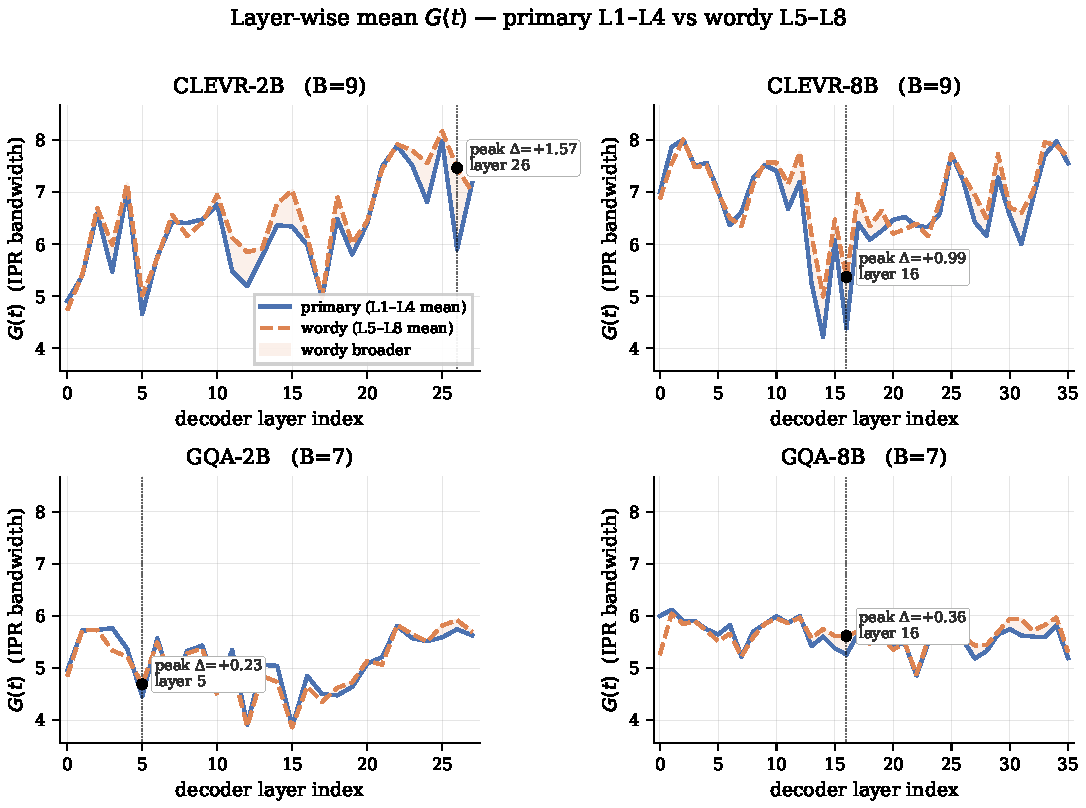
\includegraphics[width=\linewidth]{n1_trajectory_grid.pdf}
    \end{column}
    \begin{column}{0.42\textwidth}
      \small
      Four-stage trajectory in all runs:
      \begin{enumerate}\small
        \item \textbf{Layer 0:} length prior (verbose $<$ terse)
        \item \textbf{Early:} prior erasure
        \item \textbf{Mid:} $\Csem$-driven narrowing
        \item \textbf{Late:} verbosity \textbf{widening}
      \end{enumerate}
      \medskip
      \centering\scriptsize
      \begin{tabular}{lcc}
        \toprule
        & \multicolumn{2}{c}{$\Gt$ at last\_2}\\
        Run & terse & verbose \\
        \midrule
        CLEVR-2B & 5.90 & \textbf{7.47} \\
        GQA-8B   & 5.82 & \textbf{5.97} \\
        \bottomrule
      \end{tabular}
    \end{column}
  \end{columns}
\end{frame}

% ---- P2 mechanism ----
\begin{frame}{P2 --- Narrow vs.\ broadband filters drift differently}
  \begin{columns}[T]
    \begin{column}{0.62\textwidth}
      \centering
      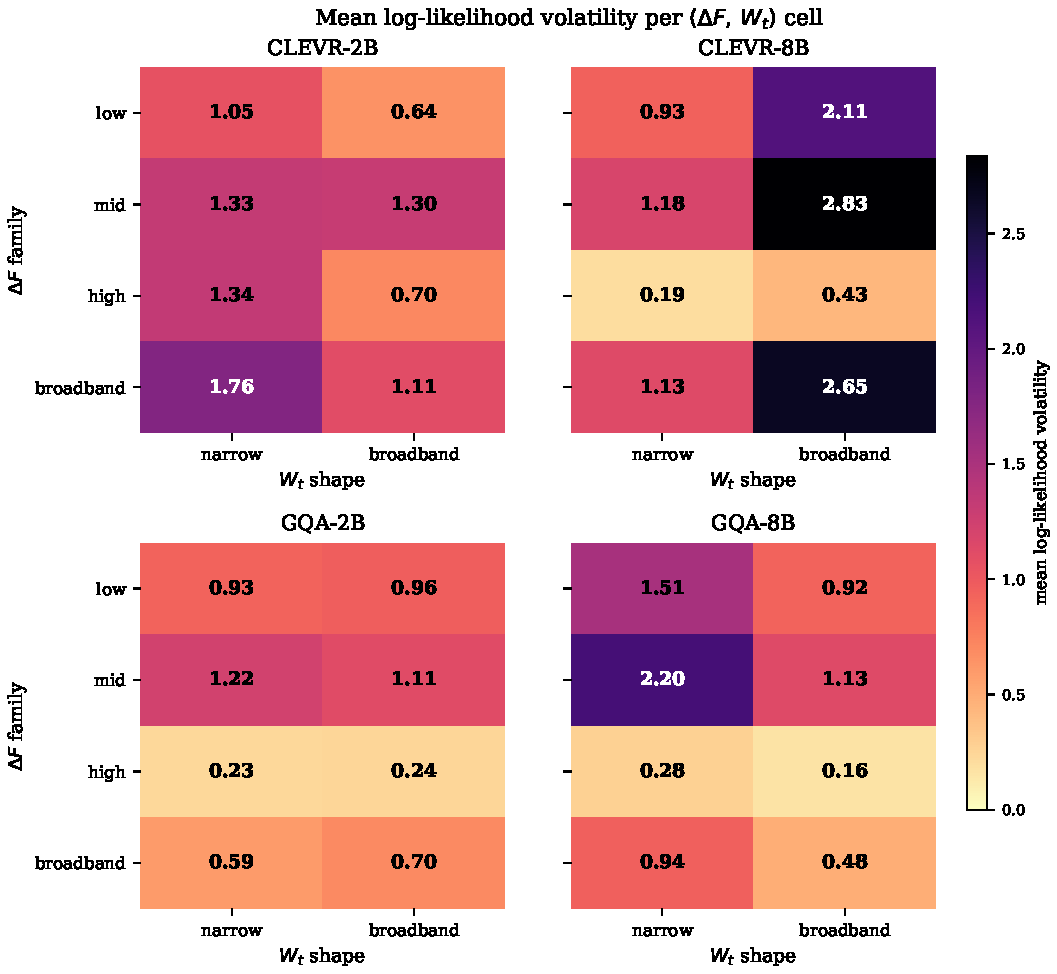
\includegraphics[width=\linewidth]{n2_signature_matrices_grid.pdf}
    \end{column}
    \begin{column}{0.38\textwidth}
      \small
      Narrow-$\Wt$ tasks lose more on a band-matched perturbation than
      broadband-$\Wt$ tasks.

      \medskip
      \cmark\ Narrow $>$ broadband in \textbf{4/4} rows on CLEVR-2B and GQA-8B.

      \medskip
      \footnotesize\textcolor{pgray}{CLEVR-8B reverses --- the recovery-dominance
      regime where verbose mirrors sit at the log-prob ceiling.}
    \end{column}
  \end{columns}
\end{frame}

% ---- P3 ----
\begin{frame}{P3 --- The overlap law predicts drift}
  \begin{columns}[T]
    \begin{column}{0.5\textwidth}
      \centering
      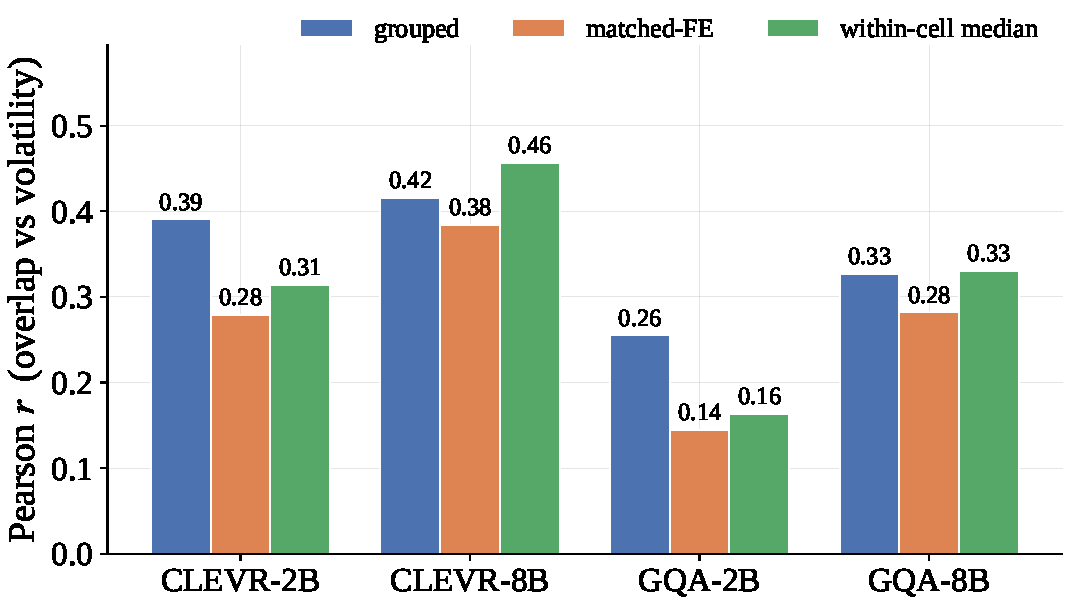
\includegraphics[width=0.96\linewidth]{n3_overlap_law_bars.pdf}
    \end{column}
    \begin{column}{0.5\textwidth}
      \centering\small
      \begin{tabular}{llccc}
        \toprule
        Model & Bench & grp & FE & cell \\
        \midrule
        Qwen-2B & CLEVR & $.39$ & $.28$ & $.31$ \\
        Qwen-8B & CLEVR & $.42$ & $.38$ & $.46$ \\
        Qwen-2B & GQA   & $.26$ & $.15$ & $.16$ \\
        Qwen-8B & GQA   & $.33$ & $.28$ & $.33$ \\
        \bottomrule
      \end{tabular}
      \medskip

      \cmark\ \textbf{Positive in 12/12} (run $\times$ aggregation) cells,
      $p\approx0$ everywhere.

      \medskip
      \footnotesize Parameter-free: no behavioural calibration.
      Grouped $r$ ranges $0.26$--$0.42$.
    \end{column}
  \end{columns}
\end{frame}

% ---- P4 ----
\begin{frame}{P4 --- High-frequency noise is \emph{not} the hard case}
  \begin{columns}[T]
    \begin{column}{0.58\textwidth}
      \centering
      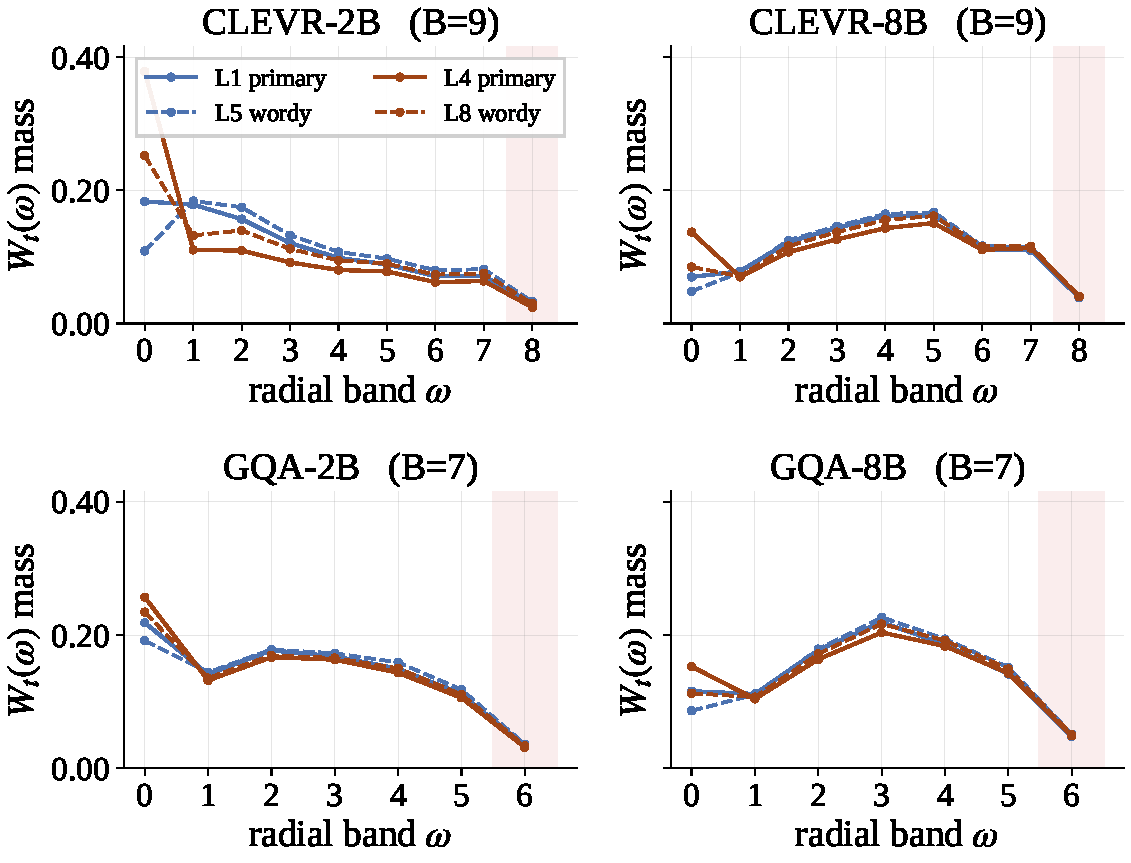
\includegraphics[width=\linewidth]{n4_band_mass.pdf}
    \end{column}
    \begin{column}{0.42\textwidth}
      \small
      Common assumption: VLMs are most vulnerable to high-frequency noise.

      \medskip
      \textbf{We find the opposite:}
      \begin{itemize}\small
        \item Most real perturbations are \textbf{low-frequency}.
        \item $\Wt$ puts only \textbf{3--5\%} mass on the top band.
        \item $\Rightarrow$ high-freq corruptions cause the \textbf{smallest}
              drift in 3/4 runs.
      \end{itemize}
      \medskip
      \footnotesize\textcolor{pgray}{What older work calls ``high'' is our mid-band.}
    \end{column}
  \end{columns}
\end{frame}

%==============================================================================
\section{Cross-architecture}

\begin{frame}{The framework is architectural, not Qwen-specific}
  Same pipeline on \textbf{LLaVA-OneVision-0.5B} (SigLIP + Qwen2, no CLS, $B=20$),
  GQA, 500 images.
  \vfill
  \centering\small
  \begin{tabular}{lccc}
    \toprule
    & Qwen-2B & Qwen-8B & LLaVA-OV-0.5B \\
    & (GQA) & (GQA) & (GQA) \\
    \midrule
    Overlap $r$ (last\_2)          & $+0.255$ & $+0.327$ & \textbf{$+0.343$} \\
    last\_2 $\Gt$ terse/verbose    & 5.75/5.92 & 5.82/5.97 & 15.72/\textbf{16.28} \\
    $\tilde\beta_{\Cprompt}$       & $-0.289$ & $-0.623$ & $-0.140$ \\
    Top-band mass                  & 3--5\% & 3--5\% & $<1\%$ \\
    \bottomrule
  \end{tabular}
  \vfill
  \keybox{\centering All four predictions replicate on a different VLM family ---
  the trajectory, overlap law, cutoff, and the verbose/complexity signs.}
\end{frame}

%==============================================================================
\section{Takeaways}

\begin{frame}{What this buys you}
  \begin{itemize}
    \item \textbf{A mechanism, not just a benchmark:} robustness is governed by
          spectral alignment between a prompt-induced filter and the corruption.
    \item \textbf{A parameter-free predictor:} $\langle\Wt,\DF\rangle$ forecasts
          drift from model internals --- no held-out calibration.
    \item \textbf{A reframed cutoff law:} low-frequency, not high-frequency,
          corruptions dominate VLM fragility.
    \item \textbf{A free robustness lever:} verbose paraphrasing reduces drift
          variance by \textbf{70--81\%} on the 8B model.
  \end{itemize}
  \vfill
  \keybox{\centering\large \textcolor{paccent}{\textbf{Pad the prompt.}}}
\end{frame}

\begin{frame}{Limitations \& honesty}
  \begin{itemize}
    \item Results on Qwen3-VL-\{2B, 8B\}; LLaVA-OneVision is a
          \textbf{single-condition} cross-architecture check (0.5B, GQA only).
    \item Some gates hold cleanly only on 8B (signed-drift reverses on CLEVR-8B
          under recovery dominance).
    \item Overlap law stronger on CLEVR; cutoff law cleaner on GQA.
    \item $\Wt$ is read from attention scores --- a \textbf{correlational}
          lower bound on the causal filter.
    \item Verbose mirrors are programmatic; human paraphrases are future work.
  \end{itemize}
\end{frame}

\begin{frame}[standout]
  Cross-modal attention is a frequency filter.\\[6pt]
  Verbose prompts broaden it; fine reasoning narrows it;\\
  overlap with the corruption controls drift.\\[12pt]
  \textbf{Pad the prompt.}
\end{frame}

%==============================================================================
\appendix

\begin{frame}{Backup --- the pipeline, end to end}
  \centering
  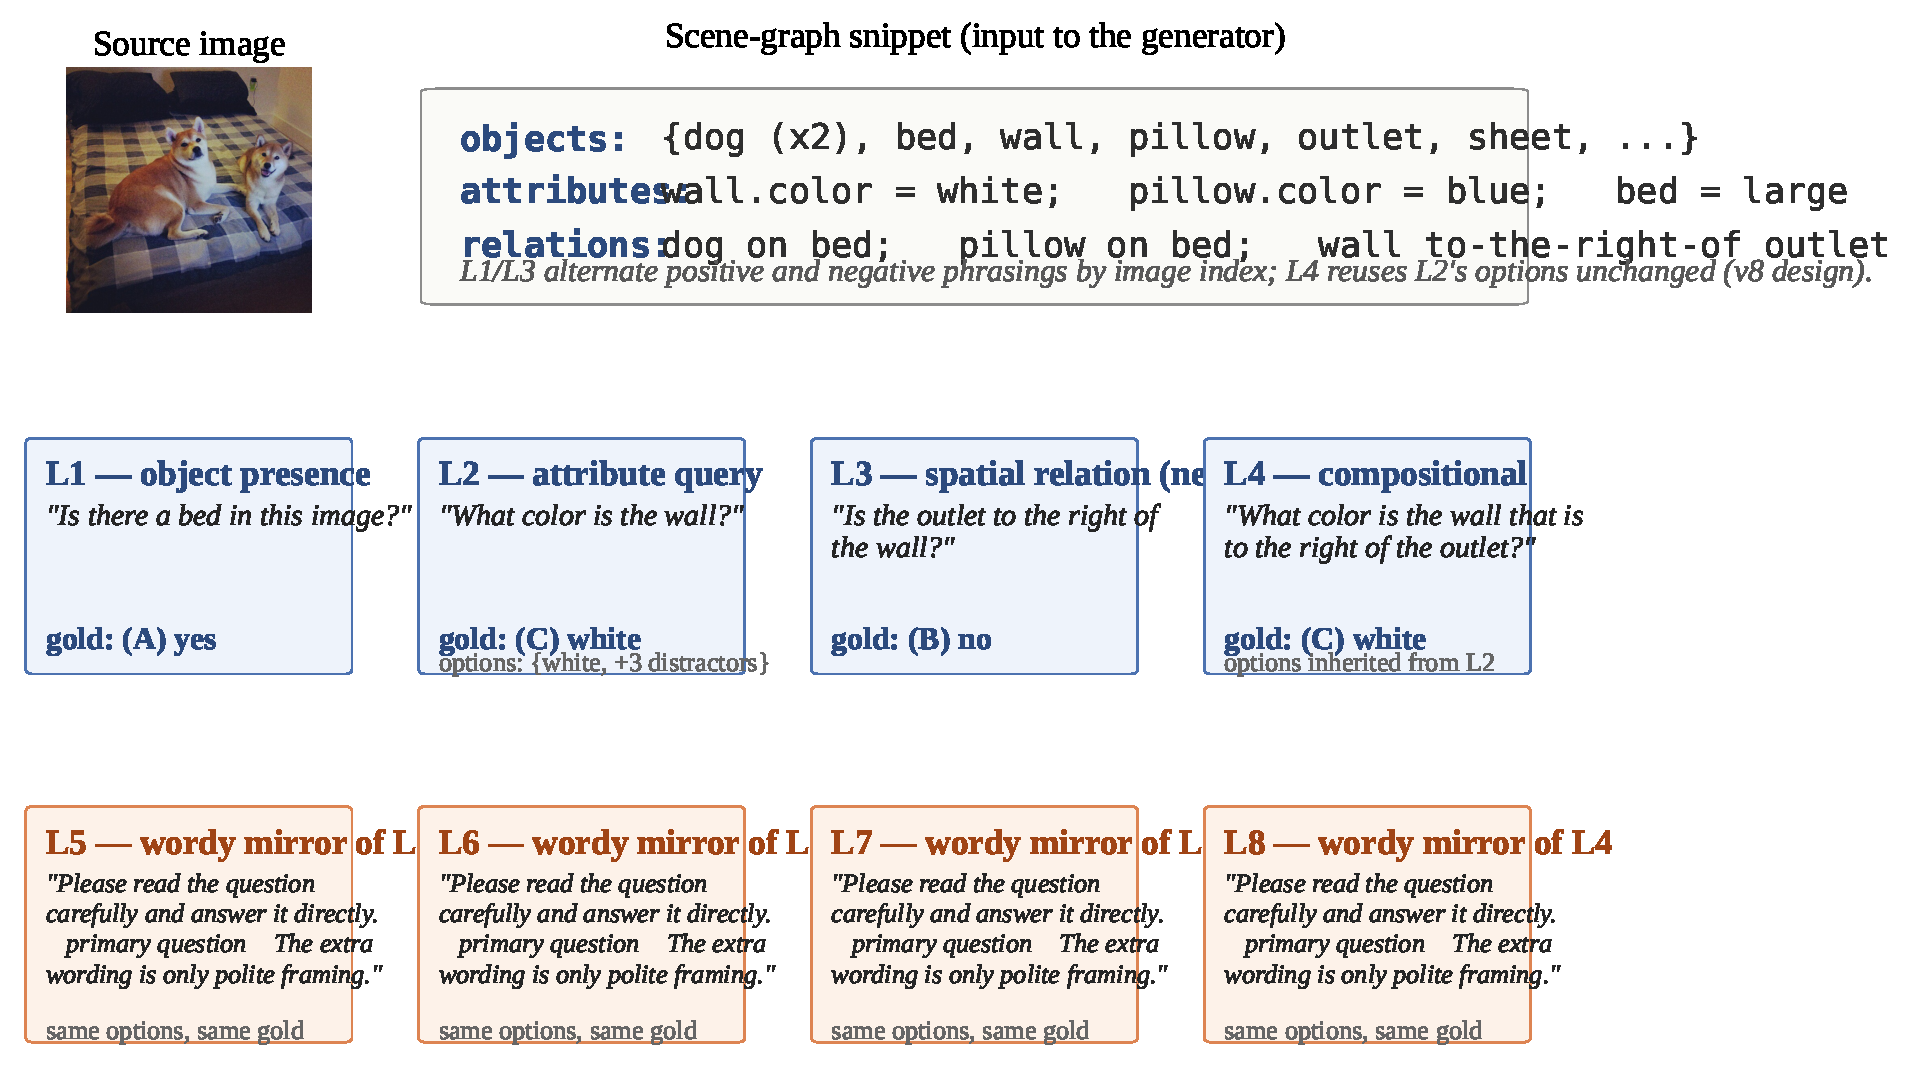
\includegraphics[width=0.92\linewidth]{appendix_pipeline.pdf}
\end{frame}

\begin{frame}{Backup --- designed vs.\ measured spectral signatures}
  \centering
  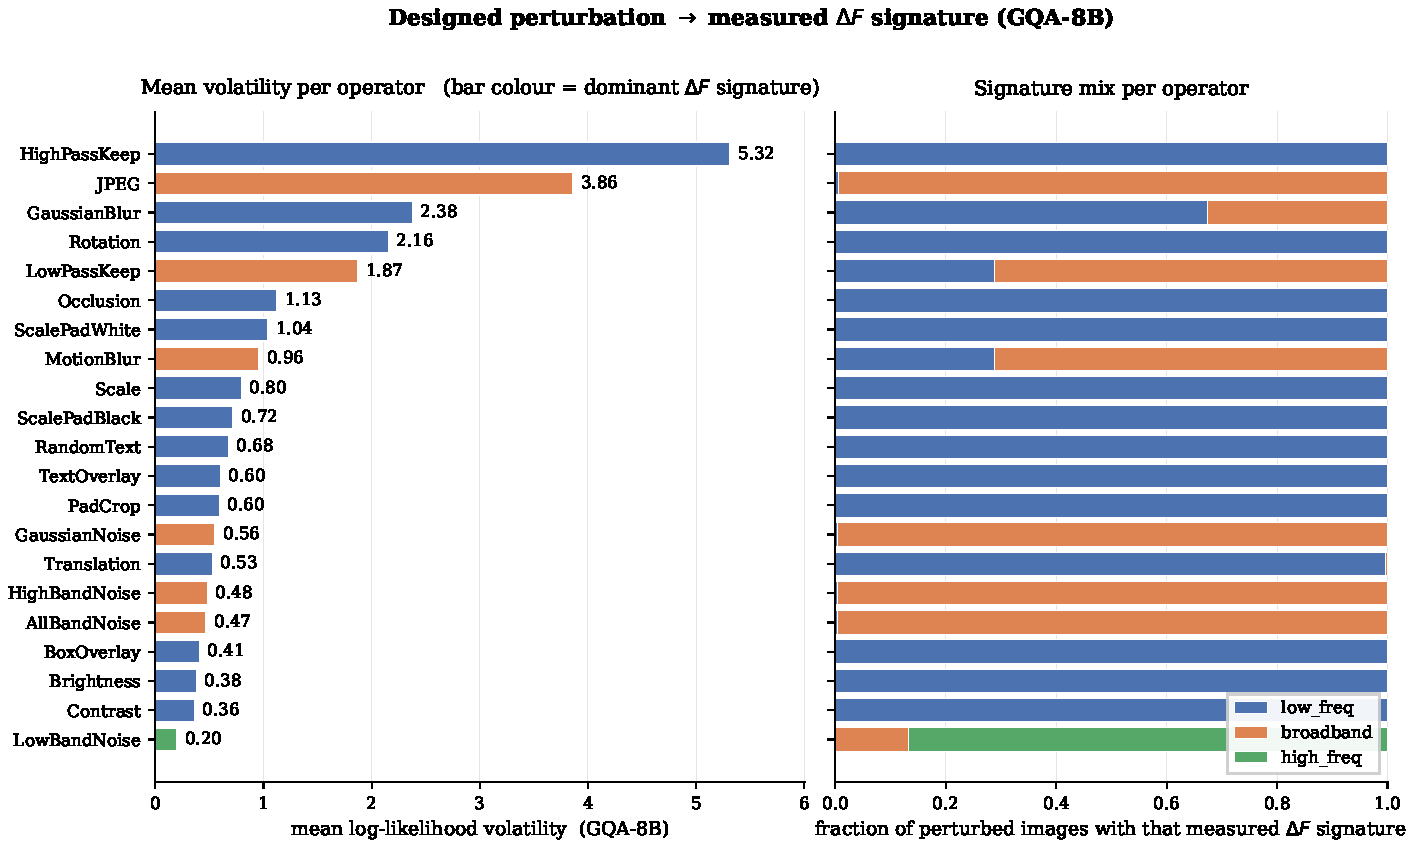
\includegraphics[width=0.74\linewidth]{n5_designed_vs_actual.pdf}\\
  \scriptsize\textcolor{pgray}{All analyses condition on the \emph{measured} $\DF$,
  not the operator's nominal name.}
\end{frame}

\begin{frame}{Backup --- worked example (one GQA image)}
  \begin{columns}[c]
    \begin{column}{0.5\textwidth}
      \centering \footnotesize Clean\\
      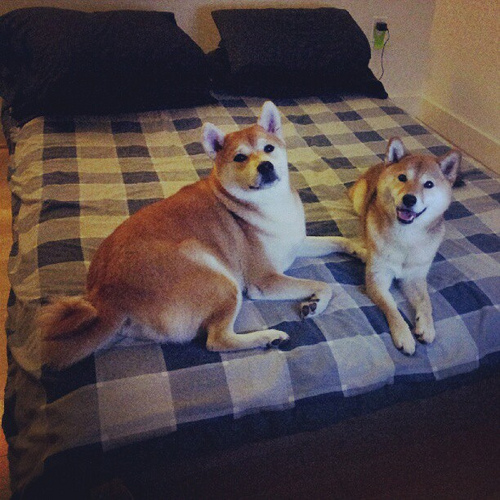
\includegraphics[width=0.82\linewidth]{example_gqa_clean.png}
    \end{column}
    \begin{column}{0.5\textwidth}
      \centering \footnotesize \texttt{Translation(+4)}\\
      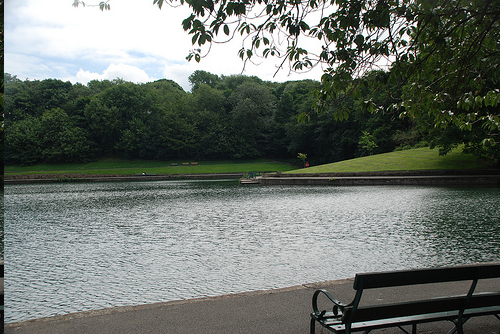
\includegraphics[width=0.82\linewidth]{example_gqa_pert.png}
    \end{column}
  \end{columns}
  \scriptsize\textcolor{pgray}{Verbose mirrors arrive near $0$ nat; terse primaries up to $19$ nat lower ---
  motivating within-cell volatility as the analysis target.}
\end{frame}

%==============================================================================
\section{Future directions}

% ---- Proposal 1 ----
\begin{frame}{Direction 1 --- Spectral attention control for global-configuration tasks}
  \textbf{Two documented clean-image failures of VLMs:}
  \begin{itemize}\small
    \item \textbf{Visual path following:} models lose the target path and switch to
          \emph{locally similar} distractors --- ``local competition'' pulls them off
          the true continuation \\
          \textcolor{pgray}{(Hong et al., 2026; arXiv:2605.15672)}.
    \item \textbf{Analog clock reading:} models confuse hour/minute hands and miss the
          \emph{global hand configuration} (ClockBench: best model $13.3\%$ vs.\ humans
          $89.1\%$) \\
          \textcolor{pgray}{(\emph{It's Time to Get It Right}, arXiv:2603.08011;
          \emph{Lost in Time}, arXiv:2502.05092)}.
  \end{itemize}
  \vfill
  \keybox{\small \textbf{Hypothesis.} Both failures share a cause:
  attention \textcolor{paccent}{over-localises} on salient but incomplete local
  features, losing global relational context. Our work shows
  \textcolor{paccent}{narrow $\Wt$ $\to$ fragile} and
  \textcolor{pgreen}{broad $\Wt$ $\to$ robust \& higher clean confidence} ---
  suggesting a controllable lever.}
\end{frame}

\begin{frame}{Direction 1 --- Proposed test \& the honest tension}
  \begin{block}{Proposed intervention}
    Spectrally \textbf{broaden} the attention filter (shift mass toward low bands $=$
    global layout) at decode time, and measure tracing / clock-reading accuracy on
    clean images.
  \end{block}
  \medskip
  \begin{block}{\textcolor{paccent}{The open question (not assumed away)}}
    In our data, \textbf{fine-grained reasoning narrows} $\Wt$ --- it \emph{needs}
    local detail. So broadening universally risks hurting local discriminability.
    \medskip

    The real test: can we add \textbf{global awareness without losing local
    discriminability}? That trade-off \emph{is} the tug-of-war ($\Csem$ narrows vs.\
    $\Cprompt$ broadens) measured directly on a task where global structure is the
    bottleneck.
  \end{block}
\end{frame}

% ---- Proposal 2 ----
\begin{frame}{Direction 2 --- Vision's \emph{depth} advantage vs.\ its token disadvantage}
  \begin{columns}[T]
    \begin{column}{0.5\textwidth}
      \textbf{Established (width disadvantage):}
      \begin{itemize}\small
        \item Vision tokens are low information-density; VLMs need \emph{many} of them.
        \item Attention to vision tokens \emph{drops} during text generation
              \textcolor{pgray}{(e.g.\ arXiv:2411.03312)}.
      \end{itemize}
      \medskip
      \textbf{Underexplored (depth):}
      \begin{itemize}\small
        \item Visually-grounded predictions \textbf{stabilise by middle layers} ---
              $\sim$layer 16 (POPE, Y/N), $\sim$20 (GQA) of $\sim$29.
        \item Visual representations become \emph{interchangeable} across deeper layers
              once stabilised (logit-lens / early-exit studies).
      \end{itemize}
    \end{column}
    \begin{column}{0.5\textwidth}
      \keybox{\small \textbf{Reframing hypothesis.}
      Vision's \textcolor{paccent}{width} disadvantage (more tokens) may be partly
      offset by a \textcolor{pgreen}{depth} advantage --- fewer \emph{layers} needed
      for a visually-grounded answer $\Rightarrow$ early-exit compute savings.}
      \medskip

      \footnotesize\textbf{Link to our P2:} the attention filter $\Wt$
      \emph{stabilises its shape by mid/late layers} --- visual processing largely
      completes before the final layers, consistent with early convergence.
    \end{column}
  \end{columns}
\end{frame}

\begin{frame}{Direction 2 --- Proposed measurements}
  \begin{enumerate}
    \item \textbf{Per-layer answer stability:} logit-lens the gold answer at every layer;
          find the depth $\ell^\star$ where the prediction stops changing, separately for
          \emph{vision-grounded} vs.\ \emph{text-only} items.
    \item \textbf{Filter convergence depth:} the layer where $\Wt$'s shape (bandwidth
          $\Gt$, band-mass) stops moving --- does it coincide with $\ell^\star$?
    \item \textbf{Width--depth trade-off:} under a fixed compute budget, trade vision-token
          count (width) against layers used (depth); map the Pareto frontier.
  \end{enumerate}
  \vfill
  \keybox{\centering \small If visually-grounded answers converge early, \textbf{early exit
  on vision-heavy items} recovers compute that the token disadvantage spends ---
  a depth-side answer to a width-side problem.}
\end{frame}

\begin{frame}[standout]
  Two levers from one mechanism:\\[6pt]
  \textcolor{pgreen}{broaden} the filter for global-configuration tasks,\\
  \textbf{exit early} where the filter has already converged.\\[10pt]
  \footnotesize\textcolor{pgray}{Both testable with the tools in this paper.}
\end{frame}

\end{document}
